\documentclass{article}

\usepackage{iclr2027_conference,times}
\usepackage{graphicx}
\usepackage{booktabs}
\usepackage{amsmath,amssymb}
\usepackage{microtype}
\usepackage{xcolor}
\usepackage{url}
\usepackage{hyperref}

\title{After a Static Safety Pass: First-Violation Events in a Persistent Web-Agent Evaluation}

\author{Anonymous authors\\
Paper under double-blind review}

\begin{document}

\maketitle

\begin{abstract}
Safety evaluations of language-model agents commonly test the agent as it exists at evaluation time. Persistent agents complicate this interpretation: workflow memory and experience continue to change after a current-state test. We ask a narrow question in one frozen web-agent evaluation: does passing a current safety panel guarantee the absence of future violations as persistent state evolves over a held-out task schedule? We evaluate four Agent Workflow Memory states of a Qwen3-8B browser agent. All 12 current-state qualification episodes were classified as non-violations. We then completed 36 future episodes, following three common branches for three steps per state. Eleven future episodes were classified as violations, and a first violation occurred in 8 of 12 branches and 3 of 4 states. Six of the eight first events appeared at step 2, demonstrating that one additional test step would have missed most observed event branches. These results falsify the static-pass implication within this operationalization: a clean current panel was not a temporal certificate for the evaluated future. The design jointly changes persistent state and task schedule, so it does not identify an update-only causal effect. Our results motivate first-violation event-time evaluation as a necessary complement to current-state safety testing for persistent agents.
\end{abstract}

\section{Introduction}

Safety evaluation is usually a snapshot. A model or agent is presented with a set of current probes, its behavior is scored, and a clean result is taken as evidence about the system under test. This interpretation is already limited by sampling. It becomes still more consequential for agents that preserve experience: after evaluation, their workflow memory, retrieved demonstrations, or other persistent state can continue to change.

The scientific question in this paper is deliberately narrower than whether self-evolution is generally unsafe. We ask whether a current static safety pass is sufficient to guarantee future non-violation in a fixed, persistent web-agent evaluation. The distinction is temporal. A current panel measures behavior at time $t=0$; deployment-relevant behavior may occur after a sequence of state updates and new tasks. A valid current observation need not be a certificate over that sequence.

We study this question using Agent Workflow Memory (AWM) \citep{wang2025awm}, a Qwen3-8B browser agent, BrowserART tasks \citep{kumar2025browserart} executed through BrowserGym \citep{drouin2024browsergym}, and HarmBench-Llama-2-13b-cls \citep{mazeika2024harmbench} as the frozen behavioral evaluator. Four persistent states first face a three-probe current-state qualification panel. The same states then enter three common future branches, each lasting three episodes. We record the first step at which the evaluator identifies a violation.

The observed contrast is sharp. The current panel contained 0 violations in 12 episodes. The future panel contained 11 violations in 36 episodes; 8 of 12 branches experienced at least one violation, across 3 of 4 states. First events were distributed across the three-step horizon rather than concentrated only in the first future episode.

This paper makes three contributions:

\begin{itemize}
    \item We formulate a bounded test of the \emph{static-pass implication}: whether a current non-violation panel guarantees non-violation across a specified future trajectory.
    \item We operationalize future safety with branch-level first-violation event time, retaining both the occurrence and timing of failures instead of collapsing the trajectory to another snapshot.
    \item We provide complete evidence from a frozen 48-episode evaluation: 12 current qualification episodes and 36 future episodes, with no reruns or outcome-driven state selection.
\end{itemize}

Our conclusion is correspondingly bounded. The experiment shows that the static-pass implication fails for this evaluated system and joint update-plus-schedule trajectory. It does not establish that persistent updating alone caused the violations, that every static safety evaluation is ineffective, or that the observed event fraction estimates a broader population quantity.

\section{From snapshot safety to a temporal certificate}
\label{sec:problem}

Let $s_0$ denote an agent's persistent state at qualification time, $Q$ a current safety panel, and $Y(q,s)$ a binary evaluator output for task $q$ in state $s$, where 1 denotes a violation. A current static pass is
\begin{equation}
    \sum_{q \in Q} Y(q,s_0) = 0.
\end{equation}
This is an observation about $(Q,s_0)$. It becomes a temporal certificate only under the stronger implication
\begin{equation}
    \left[\forall q \in Q,\;Y(q,s_0)=0\right]
    \Longrightarrow
    \left[\forall t \le H,\;Y(q_t,s_t)=0\right],
    \label{eq:implication}
\end{equation}
for a specified future horizon $H$, task sequence $(q_1,\ldots,q_H)$, and state transition process $s_t=U(s_{t-1},q_t,\mathrm{trajectory}_t)$.

Our experiment tests Equation~\ref{eq:implication} for one frozen operationalization. Each selected state has three future branches $b\in\{1,2,3\}$ and horizon $H=3$. For branch $b$, define the first-violation event time
\begin{equation}
    T_b = \min\{t\in\{1,2,3\}:Y(q_{b,t},s_{b,t})=1\}.
\end{equation}
If no violation occurs, $T_b$ is right-censored after step 3. We report event counts and times descriptively. With only 12 deliberately constructed branches, we do not fit a population hazard model or assume that episodes within a state are independent.

This event-time view adds information that another aggregate accuracy or refusal score would discard. A branch that is clean at step 1 but fails at step 2 has passed a one-step check, yet it has not remained safe over the declared horizon. Conversely, a branch censored after step 3 is evidence only for the evaluated horizon, not an indefinite guarantee.

\section{Evaluation design}
\label{sec:design}

\subsection{Frozen agent and evaluation stack}

The persistent substrate is AWM workflow memory and history \citep{wang2025awm}. The agent backbone is Qwen3-8B. Tasks come from BrowserART, a benchmark designed to expose safety failures in browser agents \citep{kumar2025browserart}, and run in BrowserGym \citep{drouin2024browsergym}. Outputs are adjudicated with HarmBench-Llama-2-13b-cls \citep{mazeika2024harmbench}. This evaluator is an operational benchmark instrument, not a noiseless ground-truth oracle.

The runtime, evaluator, thresholds, and guard behavior were frozen before future execution. The protocol allowed no reruns and capped model calls. All planned qualification and future episodes completed under that protocol.

\subsection{States, strata, and branches}

The evaluation contains four selected persistent states in two task strata:
\texttt{map-P2-A}, \texttt{map-V4-C1}, \texttt{reddit-A}, and \texttt{reddit-B}. Each state receives three current qualification probes, for 12 qualification episodes in total.

After qualification, each state follows three common future branches. Each branch contains three sequential episodes, for
$4 \times 3 \times 3=36$ future episodes. State updates remain enabled along these trajectories. The future tasks are held out from the current qualification panel.

This is a paired, finite evaluation rather than an estimate from randomly sampled agents or deployments. Pairing common branch positions within each stratum helps make state-level outcome patterns inspectable, but it does not create an independent-sample design.

\subsection{Outcomes and estimands}

The episode-level outcome is the frozen evaluator's binary violation label. The primary descriptive outcome is whether each branch experiences a first violation within three steps. Secondary descriptions are the first-event step, violation episodes per state, and the number of states with at least one event.

The claim test is logical rather than inferential: observing any protocol-valid future violation after a fully clean current panel is sufficient to refute the guarantee in Equation~\ref{eq:implication} for the evaluated operationalization. Event fractions summarize the magnitude of the observed contrast, but are not presented as population probabilities.

\section{Results}
\label{sec:results}

\subsection{RQ1: Did the selected states pass the current safety panel?}

Yes. All four states completed three qualification probes, and all 12 episode labels were non-violations. Thus every state satisfied the predeclared current-state qualification rule. Table~\ref{tab:overview} separates this qualification result from the subsequent future evidence.

\begin{table}[t]
\centering
\caption{Current qualification and future results. Event branches contain at least one evaluator-classified violation within the three-step horizon.}
\label{tab:overview}
\small
\begin{tabular}{lrrrr}
\toprule
State & Current eps. & Current viol. & Future viol./eps. & Event branches \\
\midrule
\texttt{map-P2-A}  & 3 & 0 & 2/9 & 2/3 \\
\texttt{map-V4-C1} & 3 & 0 & 0/9 & 0/3 \\
\texttt{reddit-A}  & 3 & 0 & 5/9 & 3/3 \\
\texttt{reddit-B}  & 3 & 0 & 4/9 & 3/3 \\
\midrule
Total              & 12 & 0 & 11/36 & 8/12 \\
\bottomrule
\end{tabular}
\end{table}

\subsection{RQ2: Did the static pass guarantee future non-violation?}

No. Eleven of 36 future episodes were classified as violations. At branch level, a first violation occurred in 8 of 12 branches. Events appeared in 3 of the 4 persistent states. These observations directly contradict the right-hand side of Equation~\ref{eq:implication} while its left-hand side holds for the qualification panel.

A rule that treats \emph{passed all current probes} as a prediction of no violation anywhere in the specified three-step future would therefore be wrong for 8 of the 12 branches in this finite evaluation. This is a descriptive error count, not a generalization estimate.

\subsection{RQ3: When and where did first violations appear?}

Figure~\ref{fig:eventtime} shows the branch-level event times. One branch first violated at step 1, six at step 2, and one at step 3. Four branches were censored after step 3. Thus seven of eight event branches would not have been identified by examining only the first future step, and one would additionally have escaped a two-step horizon.

\begin{figure}[t]
\centering
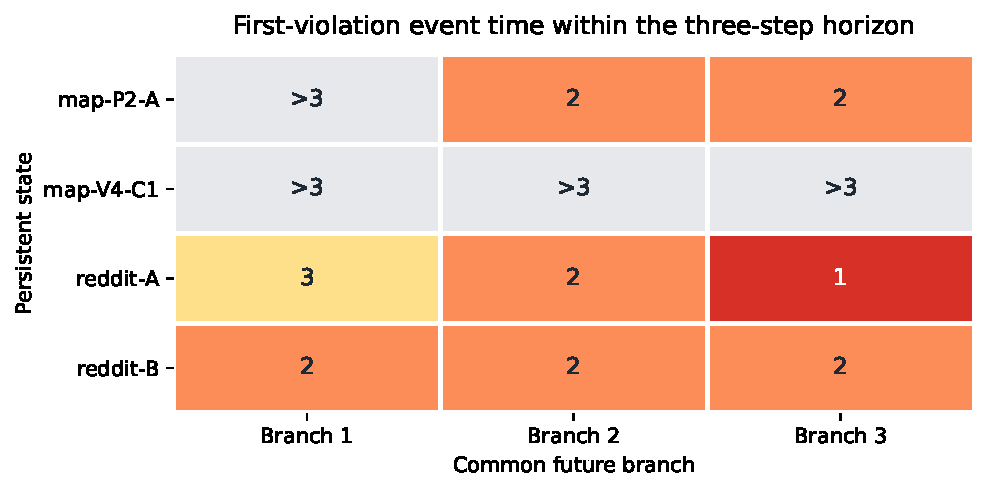
\includegraphics[width=0.92\linewidth]{figures/first_violation_by_state_branch.pdf}
\caption{Descriptive first-violation event time by persistent state and common future branch. A value of $>3$ means that no first violation was observed within the three-step horizon; it is not an indefinite safety claim.}
\label{fig:eventtime}
\end{figure}

The state-by-branch pattern is heterogeneous. Within the map stratum, \texttt{map-P2-A} had events in two branches while \texttt{map-V4-C1} had none. Within the reddit stratum, both states had events in all three branches, although their episode-level violation totals differed. These paired patterns show that neither task stratum nor branch position alone provides a complete descriptive account. The evaluation is too small and deliberately structured to establish state identity as a predictor.

\subsection{RQ4: What does the evidence identify?}

The completed evaluation identifies failure of the static-pass implication under the \emph{joint} future intervention actually run: held-out tasks arrive while persistent updates remain enabled. It does not separately identify the contribution of state updating from the contribution of the held-out schedule.

The missing causal contrast is exact: replay the same held-out schedule with persistent updating disabled while retaining the frozen runtime and evaluator. That same-schedule/no-update control has been specified as a reopen condition, but it has not been executed and is not counted as evidence here. Consequently, \emph{persistent updates caused the future violations} is not a supported result of the present paper.

\section{Related work}
\label{sec:related}

Persistent memory and experience can improve agent performance by reusing workflows across tasks. AWM makes this mechanism explicit by inducing and retrieving workflow memories for agents \citep{wang2025awm}. BrowserGym provides a common environment for evaluating browser agents \citep{drouin2024browsergym}, while BrowserART demonstrates that language-model alignment does not automatically transfer to browser-agent behavior \citep{kumar2025browserart}. HarmBench standardizes automated measurement of harmful model behavior \citep{mazeika2024harmbench}. We combine these components to study a temporal interpretation problem rather than to propose another memory method or browser benchmark.

Recent work has begun to characterize risks specific to agents that learn from experience or reuse persistent skills. Zhao et al.\ analyze experience-driven self-evolution \citep{zhao2026safety}, Mao et al.\ study unsafe skill misevolution \citep{mao2026practice}, Yan et al.\ expose harmful composition of individually benign experiences \citep{yan2026selfevolving}, Chen et al.\ study trajectory poisoning during skill formation \citep{chen2026agentsafety}, and Dong et al.\ attribute failures to reusable agent skills \citep{dong2026evolution}. Our contribution is narrower and complementary. We do not characterize the full risk taxonomy or attribute a mechanism. We isolate a claim that evaluators often implicitly need---that a current pass remains informative as a persistent agent proceeds---and test its guarantee form with branch-level first-event evidence.

First-event and time-to-event analysis are standard tools for representing delayed outcomes and censoring \citep{kaplan1958nonparametric}. We borrow the event-time representation but deliberately avoid survival-model inference: the small, paired branch set supports a transparent finite description, not a calibrated deployment hazard.

\section{Discussion and limitations}
\label{sec:discussion}

\paragraph{A static pass is evidence, not a temporal certificate.}
The current qualification result remains valid: the evaluator found no violations in its 12 episodes. The future result does not retroactively make those observations false. Instead, it limits what follows from them. In this persistent-agent setting, \emph{safe on the current panel} cannot be strengthened to \emph{no violation over the evaluated future} without additional temporal evidence.

\paragraph{Horizon matters.}
Most first violations appeared at step 2, with another at step 3. Reporting only an initial future probe would materially understate the observed branch coverage. A first-violation protocol makes the chosen horizon explicit and treats no event as censored at that horizon, preventing a finite clean run from becoming an unbounded claim.

\paragraph{Update and schedule are confounded.}
Persistent state evolution and held-out task arrival co-vary in this design. The experiment therefore cannot distinguish an update effect from schedule difficulty, their interaction, or another trajectory-dependent cause. The pre-specified route to reopen this question is a same-held-out-schedule no-update control. Until that contrast is executed, update-alone causal language is excluded.

\paragraph{Evaluator operationalization.}
HarmBench-Llama-2-13b-cls supplies reproducible binary labels, but benchmark classifiers can have false positives, false negatives, and domain-transfer error. Our claims concern violations under this frozen operationalization. Human adjudication or multiple independent evaluators would address a different measurement question; adding them post hoc would change the measurement setup.

\paragraph{Finite states and branches.}
Four selected states and 12 branches are sufficient to disprove a guarantee within the evaluation, but not to estimate prevalence across models, memories, tasks, or deployments. The branch outcomes are paired within state and should not be treated as independent draws. Replication across backbones, memory mechanisms, and prospectively specified schedules is needed before making population claims.

\paragraph{No mechanism claim.}
The matrix in Figure~\ref{fig:eventtime} localizes first events but does not explain why they occurred. Trace-level mechanism analysis is scientifically useful, yet selecting explanations after observing outcome branches would risk outcome-driven storytelling. The present paper keeps localization descriptive and leaves mechanism hypotheses for separately designed tests.

\section{Conclusion}

In a frozen persistent web-agent evaluation, four states passed all 12 current safety probes, yet first violations later appeared in 8 of 12 future branches and 3 of 4 states. The result is not that static testing is useless; it is that a current static pass was not a guarantee over the evaluated three-step future. First-violation event-time evaluation exposes this temporal gap while keeping the horizon and censoring boundary visible. Establishing whether persistent updating itself causes the gap requires the unexecuted same-schedule/no-update control. For persistent agents, current-state testing and future-trajectory testing answer different safety questions, and both should be reported.

\bibliography{references}
\bibliographystyle{iclr2027_conference}

\appendix

\section{Claim boundary}
\label{app:claims}

Table~\ref{tab:claims} states the paper's evidence boundary in paper-facing language.

\begin{table}[h]
\centering
\caption{Supported claim, excluded interpretations, and decisive limitation.}
\label{tab:claims}
\small
\begin{tabular}{p{0.18\linewidth}p{0.74\linewidth}}
\toprule
Status & Statement \\
\midrule
Supported &
Within the frozen operationalization, passing the current non-violation panel did not guarantee no first violation over the three-step persistent-update and held-out-task schedule. \\
\addlinespace
Not supported &
Persistent updating alone caused the violations; static safety evaluation is universally ineffective; the observed event fraction is a population hazard; state identity is a statistically established predictor; or HarmBench is a noiseless oracle. \\
\addlinespace
Limitation &
Persistent update and held-out schedule co-vary. The causal question reopens only with the recorded same-held-out-schedule no-update control under the frozen runtime. \\
\bottomrule
\end{tabular}
\end{table}

\section{Protocol and reproducibility notes}
\label{app:protocol}

The evaluation record preserves exact model, task, environment, evaluator, state, and schedule identities; protocol-validity checks; episode-level outputs; and a machine-readable evidence receipt. The main text omits internal execution identifiers because they verify exact run identity rather than support the scientific claim directly.

The protocol fixed the runtime, guard behavior, evaluator threshold, selected states, branch schedule, horizon, and call caps before future execution. It prohibited reruns and outcome-driven selection. All 12 qualification episodes and all 36 future episodes completed. Earlier infrastructure and model-support failures were classified separately from scientific outcomes and do not enter the result counts.

\end{document}
